\chapter{Implementierung eines Prototypen}\label{chap:implementation}
\fixme{move code listings to appendix}
In diesem Kapitel wird die Entwicklung eines auf dem zuvor ausgearbeiteten Konzept basierten Prototypen beschrieben. Dieser Prototyp enthält nicht alle im Konzept beschriebenen Anforderungen und befindet sich auch nicht in einem finalen Entwicklungsstadium, kann aber mit weiteren Entwicklungsressourcen als Grundlage für eine finale Implementierung genutzt werden. Er soll zeigen, wie sich das entworfene Konzept umsetzen lässt und die darin benutzten Technologien miteinander interagieren.

\section{Tool zum Parsen der vorhandenen UI-Struktur}
Wie in Kapitel~\ref{chap:concept} beschrieben müssen die Dateien, welche das momentane UI-Layout enthalten, in ein web-freundliches Format (JSON) übersetzt werden. Bei diesem Schritt ist es auch direkt möglich Informationen, die zukünftig nicht mehr benötigt werden, nicht mit zu übernehmen und andere Informationen in eine optimalere Struktur zu überführen. Für diesen Zweck wurde ein kleines Hilfstool in C\# geschrieben, welches sowohl die ``.dli''-Datei der Detailansicht als auch die ``.vlc''-Datei der Übersichtsliste einer einzelnen cRM-Ansicht als Input erhält und daraus eine ``.json''-Datei mit allen benötigten Informationen erstellt. Um die Anpassbar- und Wiederverwendbarkeit des Tools zu maximieren, wurde das \textbf{Visitor-Pattern} angewandt. In Abbildung~\ref{fig:web-conv_file-tree} ist der Aufbau des Tools erkennbar.

\begin{figure}
    \centering
    \captionsetup{justification=centering}
    \frame{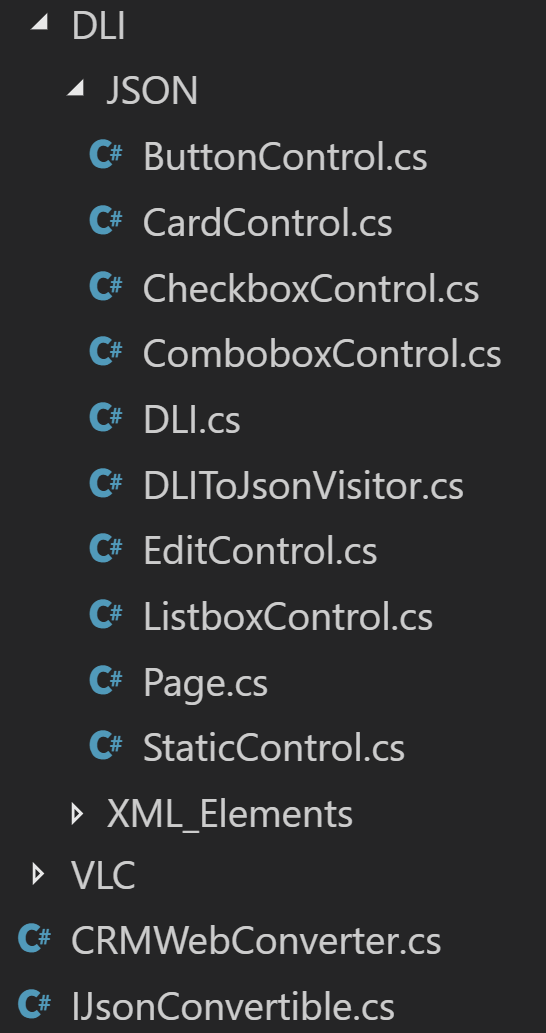
\includegraphics{figures/web-converter_file-tree.png}}
        \caption{Datei-Struktur des Konvertierungstools}\label{fig:web-conv_file-tree}
\end{figure}

Zunächst wird für jedes einzulesende Token (XML-Element) eine Klasse vom \nameformat{Acceptor}-Interface (\nameformat{IDLIAcceptor} / \nameformat{IVLCAcceptor}) abgeleitet, dieses Interface enthält eine einzige Methode \textbf{Apply}, welche einen Visitor (\nameformat{IDLIVisitor} / \nameformat{IVCLVisitor}) übergeben bekommt. Die jeweiligen Token-Klassen werden mit dem von ihnen verwalteten XML-Element (\nameformat{XElement}) initialisiert. Wie im Quellcodeauszug~\ref{lst:pageelement_init} anhand der Klasse \nameformat{PageElement} beispielhaft zu sehen, werden aus diesem XML-Element die relevanten Informationen über das Element selbst (Name und Metadaten) und dessen verschachtelte Kinder-Elemente (Liste von Controls) ausgelesen.

\lstinputlisting[language={[Sharp]C},label={lst:pageelement_init},caption={Initialisierung der PageElement-Klasse}]{code/chapter_005_pageelement_init.cs}

Nachdem die Informationen der XML-Datei auf diese Art und Weise in ihre einzelnen Token-Instanzen übersetzt wurden, wird die \textbf{Apply}-Methode, zu sehen in Quellcodeauszug~\ref{lst:dialogelement_apply}, des zentralen Tokens (\nameformat{DialogElement}) mit einer Visitor-Instanz aufgerufen. Der Visitor erhält als Parameter eben diese Instanz und extrahiert alle für ihn relevanten Informationen. Anschließend ruft er rekursiv die \textbf{Apply}-Methoden der Kinder-Token auf und liest auch aus diesen die relevanten Informationen aus. Diese Aufrufe sind im Quellcodeauszug~\ref{lst:json-visitor_visit-methods} zu sehen. Nachdem alle Tokens vollständig besucht wurden können die gewonnenen Daten als JSON-String ausgegeben werden.

\lstinputlisting[language={[Sharp]C},label={lst:dialogelement_apply},caption={Apply-Methode der DialogElement-Klasse}]{code/chapter_005_dialogelement_apply.cs}

\lstinputlisting[language={[Sharp]C},label={lst:json-visitor_visit-methods},caption={Ablaufen und Extrahieren relevanter Informationen aus XML-Tokens durch den JSON-Visitor}]{code/chapter_005_json-visitor_visit-methods.cs}

Die Flexibilität dieser Architektur, welche in der Abbildung~\ref{fig:web-conv_class-diagramm} nochmals übersichtlich als Klassendiagramm dargestellt wird, ist ebenso daran zu erkennen, dass der einzige Unterschied beim Auslesen von Detailansicht-Datei und Übersichtslisten-Datei in der Implementierung der Interfaces besteht. Sowohl \nameformat{Acceptor}- als auch \nameformat{Visitor}-Klassen können sehr leicht einzeln angepasst oder ersetzt werden. Ebenso ist es möglich weitere Tokens, welche eventuell zu einem späteren Zeitpunkt benötigt werden, aus den XML-Dateien auszulesen, indem weitere \nameformat{Acceptor}- und \nameformat{Visitor}-Implementierungen hinzufügt werden.

\begin{figure}
    \centering
    \captionsetup{justification=centering}
    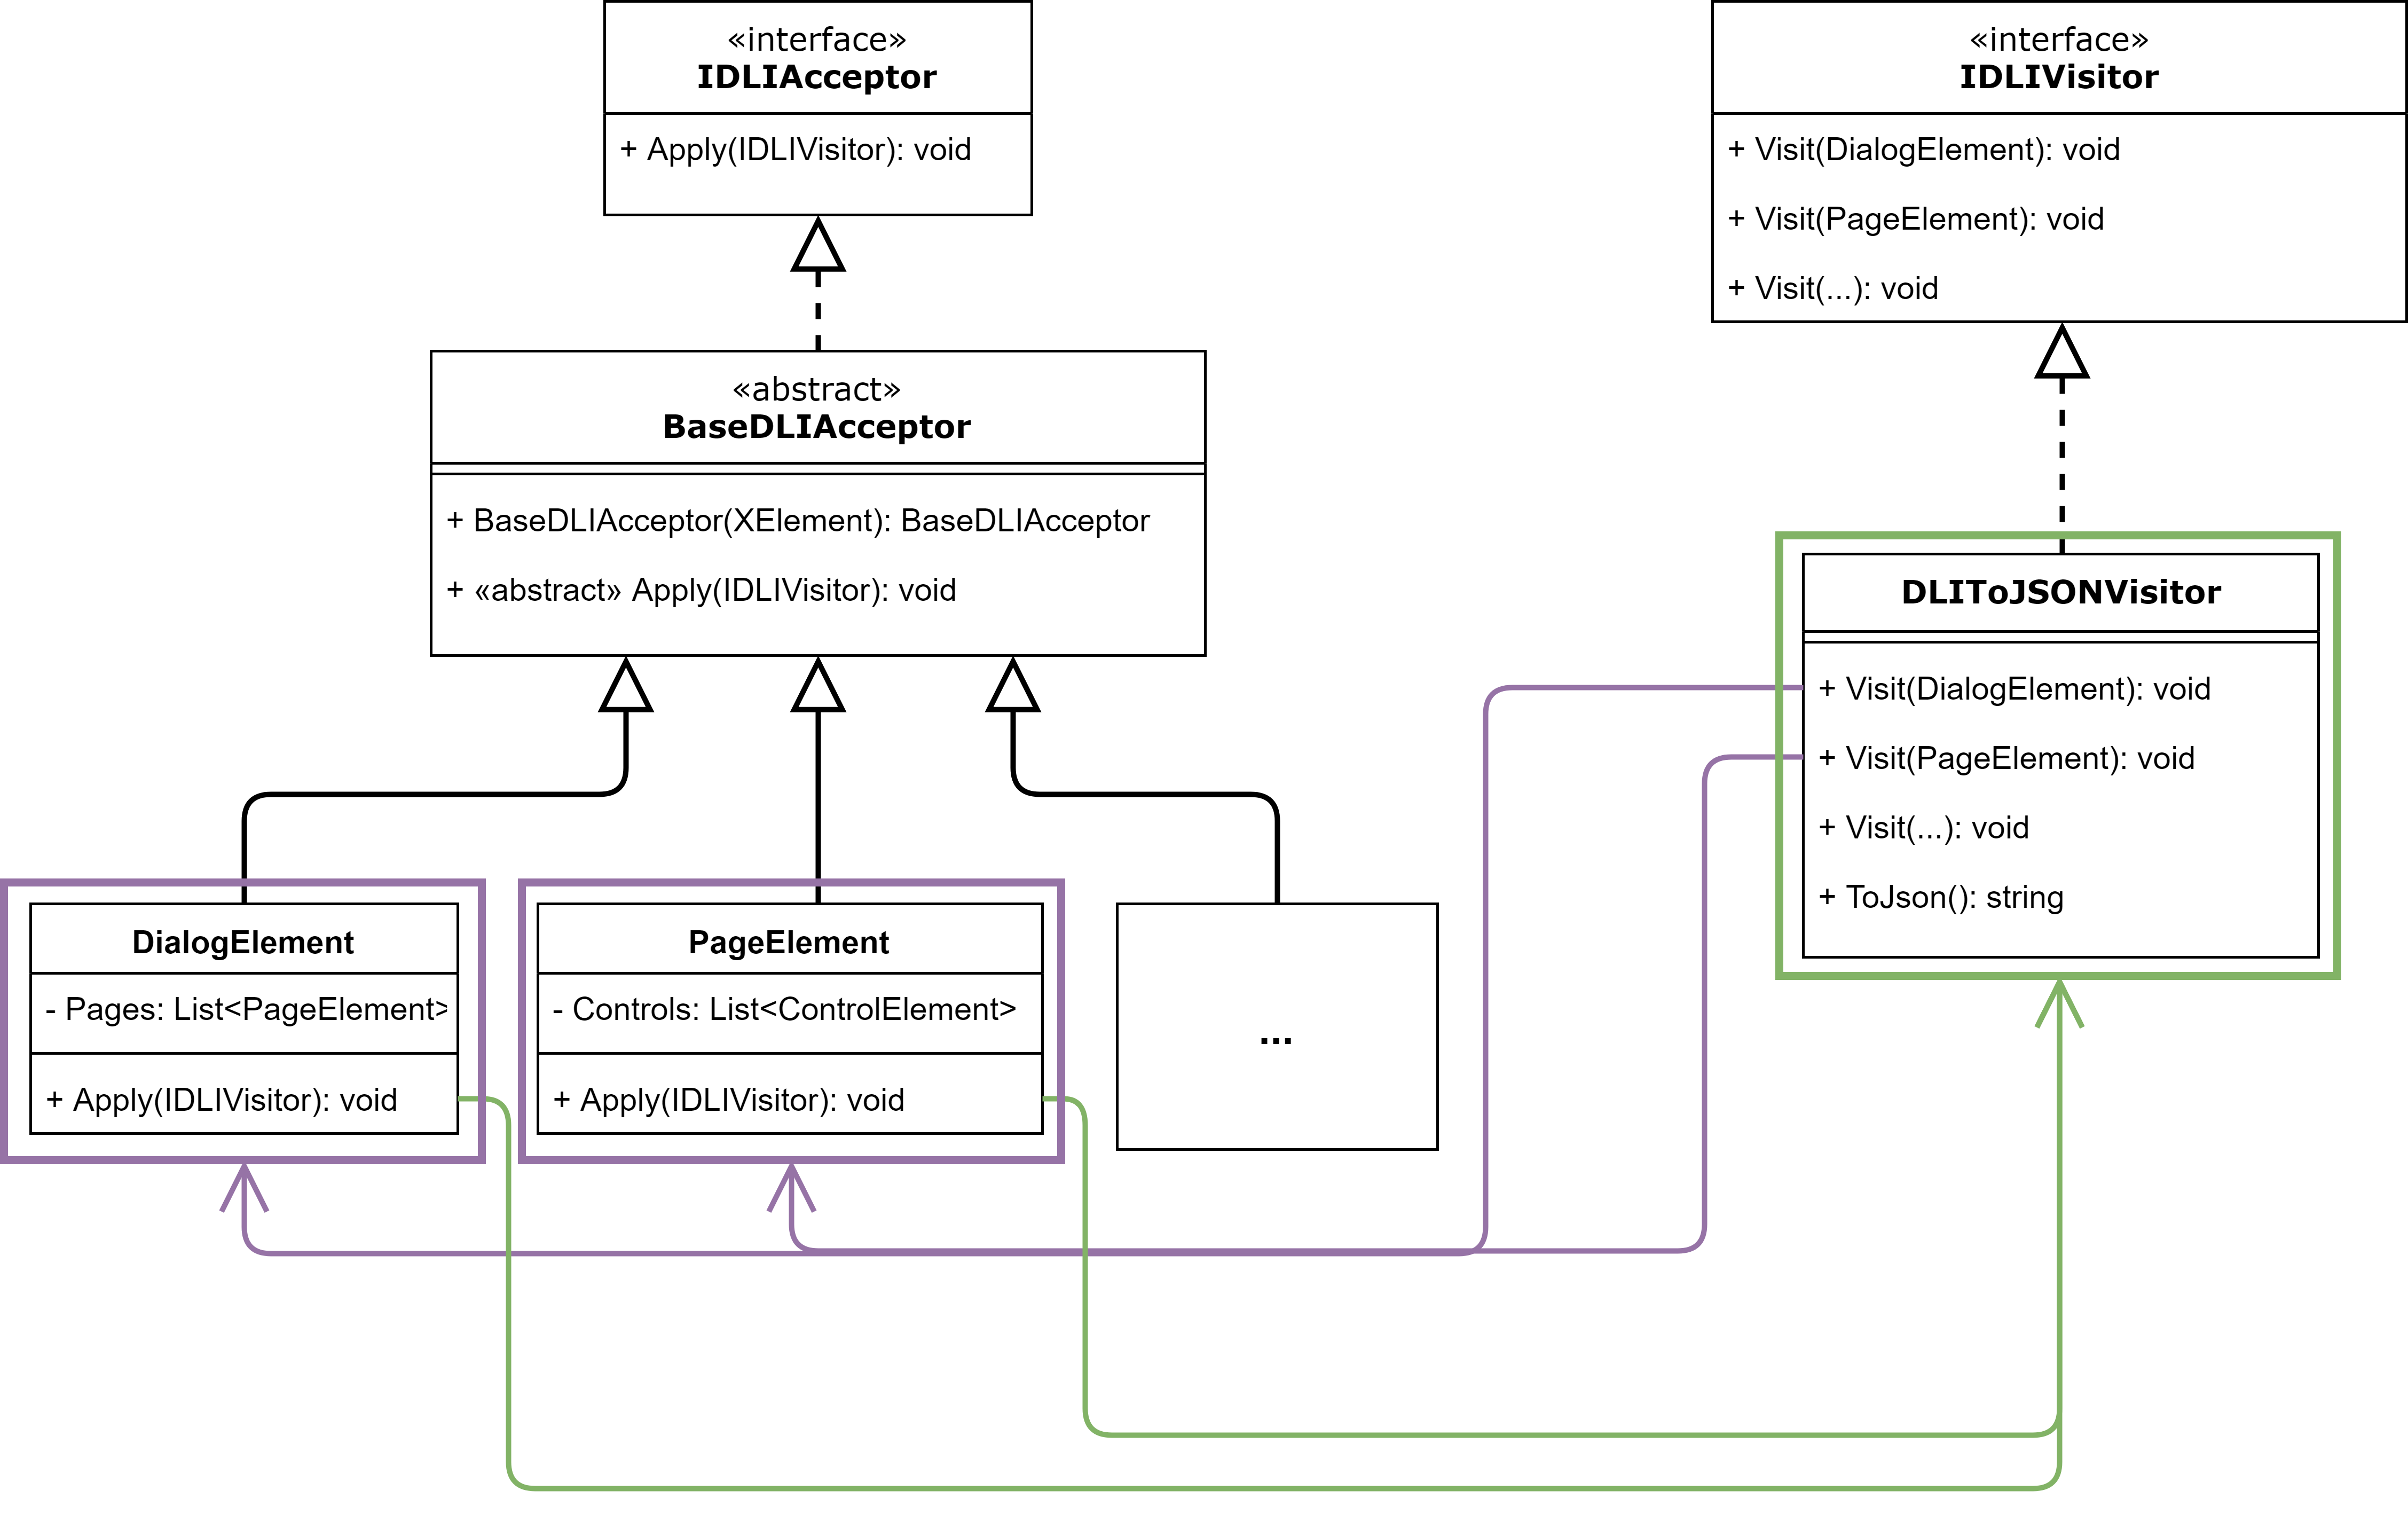
\includegraphics[width=\textwidth]{figures/web-converter_class-diagramm.png}
        \caption{Klassendiagramm der Visitor-Struktur des Konvertierungstools}\label{fig:web-conv_class-diagramm}
\end{figure}

Der Input und das Endergebnis in Form eines vom \nameformat{GraphQL}-Server direkt verwertbaren JSON-Dokument ist in Quellcodeauszug~\ref{lst:xml_input} und Auszug~\ref{lst:json_output} anhand eines kleines Auszuges ersichtlich.

\lstinputlisting[language={XML},caption={XML-Input},label={lst:xml_input}]{code/chapter_005_xml_input.xml}

\lstinputlisting[caption={JSON-Ergebnis},label={lst:json_output}]{code/chapter_005_json_output.json}

\section{Webseite}
% CRA-Skelett
% auf finalen Aufbau warten
\fixme{once project is ``final'' (Beispielumsetzung)}

\subsection{React-Komponenten}
Der Aufbau aller Komponenten folgt einem identischen Schema. Zunächst ist eine \nameformat{React}-Komponente so definiert, dass sie als Parameter alle notwendigen Eigenschaften zur Anzeige und Mutation von Daten übergeben bekommt. Die Komponente enthält keine Logik zur Veränderung der Parameter.
CSS wird mithilfe der Bibliothek \nameformat{styled-components} in Form eines Wrappers um das eigentlich anzuzeigende HTML-Tag eingesetzt. Ein Nachteil von traditionellem CSS-Einsatz ist, dass CSS-Klassen an vielen Stellen der Oberfläche eingesetzt werden und eine Änderung am Aussehen durch den fehlenden Überblick aller Stellen möglicherweise ungewollte Auswirkungen haben kann. Durch die Verknüpfung von CSS mit \nameformat{React}-Komponenten kann sich eine Änderung immer nur auf diese eine Komponente auswirken. In Ausschnitt~\ref{lst:styled_components} ist die Benutzung und Unterstützung von Themes von \nameformat{styled-components} anhand eines HTML input-Tags dargestellt.
Eine Komponente ist nicht selbst für das Abschicken der \nameformat{GraphQL}-Abfragen verantwortlich, dennoch wird der jeweilige Teil der Abfrage mit den für sie relevanten Daten zusammen mit ihr definiert. Eine speziell dafür ausgelegte Komponente weiter oben in der Hierarchie kombiniert alle Teilabfragen der UI-Komponenten (siehe Ausschnitt~\ref{lst:graphql_query}) und sendet diese an den Server. Diese Komponente ist weiterhin dafür zuständig die vom Server erhaltenen Daten wieder auf die UI-Komponenten zu verteilen.
Der vierte und letzte Bestandteil einer Komponente sind die im nächsten Abschnitt beschriebenen Tests.

\lstinputlisting[label={lst:styled_components},caption={Benutzung der styled-components Bibliothek}]{code/chapter_005_styled_components.js}

\lstinputlisting[label={lst:graphql_query},caption={Einbettung von GraphQL-Query-Fragmenten}]{code/chapter_005_graphql_query.gql}

\subsection{Tests}
Einzelne Komponenten werden durch die in Abschnitt~\ref{subsec:test_ci_concept} erwähnten Snapshot-Vergleiche (siehe Ausschnitt~\ref{lst:snapshot_test}) auf unerwünschte Veränderungen geprüft. Weiterhin wird getestet, ob die Übergabeparameter in Form von Formatierungsbedingungen oder anzuzeigenden Daten korrekt ausgewertet und dargestellt werden. Da die Clientapplikation bewusst wenig Logik enthält, werden in diesem Bereich auch verhältnismäßig wenige Tests benötigt.
Die während der Entwicklung genutzten visuellen \nameformat{Storybook}-Tests müssen für jede einzelne Komponente konfiguriert werden. Notwendig ist nur die Konfiguration der Komponente selbst, optional werden aber jeweils noch die im Produktivcode ebenso benutzte globale CSS-Deklarationen, die verfügbaren Themes und die in der UI veränderbaren Übergabeparameter (im Ausschnitt `Knobs') angegeben. Abbildung~\ref{fig:storybook_example} zeigt die Darstellung der in Ausschnitt~\ref{lst:storybook_config} gezeigten Konfiguration in der \nameformat{Storybook}-Umgebung.

\lstinputlisting[language={JavaScript},caption={Snapshot-Test mit Jest und Enzyme},label={lst:snapshot_test}]{code/chapter_005_snapshot_test.js}

\lstinputlisting[language={JavaScript},caption={Konfiguration einer Storybook Komponenten},label={lst:storybook_config}]{code/chapter_005_storybook_config.js}

\begin{figure}
    \centering
    \captionsetup{justification=centering}
    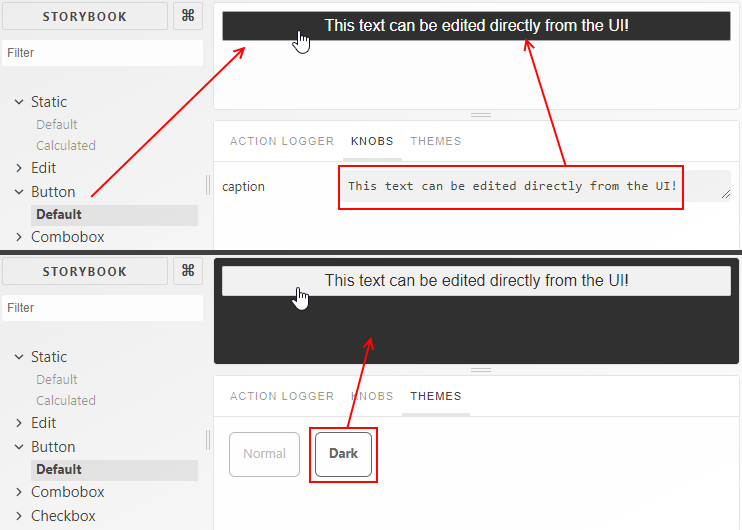
\includegraphics[width=0.8\textwidth]{figures/storybook_example.png}
        \caption{Beispiel für die Komponentendarstellung mit Storybook}\label{fig:storybook_example}
\end{figure}

\subsection{GraphQL-Mock-Server und Resolver}
Da das passende Backend zu dieser Arbeit erst zu einem späteren Zeitpunkt erstellt wird, wurde vorübergehend eine Dummy-Implementierung eines \nameformat{GraphQL}-Servers erstellt, welcher aber bereits das korrekte Schema und die Daten des erstellten Parser-Tools nutzt. Dies ermöglicht es den Client unter realen Gegebenheiten zu entwickeln. Die Implementierung besteht aus der Schemadefinition für GraphQL (einen Auszug daraus ist in Quellcodeauszug~\ref{lst:graphql_schema} zu sehen) und den Resolvern die dem Schema die konkreten Daten zuordnen (der zu Auszug~\ref{lst:graphql_schema} passende Code kann in Auszug~\ref{lst:graphql_schema_resolver} eingesehen werden). Aus diesen beiden Einzelteilen wird mithilfe der \nameformat{Apollo GraphQL-tools}~\parencite{apollo_graphql-tools_2019} ein ausführbares Schema erstellt und mit \nameformat{express-graphql}~\parencite{express_graphql_2018} lokal gehostet. Für im Schema definierte Typen, welche aufgrund fehlender Daten noch keine Resolver erhalten können, werden von den \nameformat{GraphQL-tools} automatisch Daten mit passenden Typen generiert.

\lstinputlisting[label={lst:graphql_schema},caption={Teil der GraphQL-Schemadefinition}]{code/chapter_005_graphql_schema.gql}

\lstinputlisting[language={JavaScript},label={lst:graphql_schema_resolver},caption={GraphQL Schema-Resolver}]{code/chapter_005_graphql_schema_resolver.js}

\section{Beispielumsetzung}
Um die Validität des Konzeptes zu belegen, wird eine beispielhafte, simple Oberfläche des \nameformat{\gls{crm}} Desktopclients in die neue Darstellung übersetzt.\\
\fixme{EINFACHES (wenig Elemente), ABER KOMPLETTES BSP für jetzige UI -> neue UI}
